\documentclass[notitlepage, a4paper, 11pt]{article}

\usepackage{geometry}
\geometry{
	a4paper,
	total={170mm,257mm},
	left=20mm,
	top=20mm,
}

\usepackage{ gensymb }
\usepackage{wrapfig}
\usepackage{xcolor}
\usepackage{graphicx}
\usepackage{amsmath}
\usepackage{listings}
\usepackage{xcolor}
\usepackage{minted}
\usepackage{tikz}
\usepackage[european resistors]{circuitikz}
\usepackage{caption}
\usepackage{subcaption}
\usepackage{hyperref}
\hypersetup{
	pdfborder = false,
	colorlinks=true,
	linkcolor=black,
	filecolor=black,      
	urlcolor=blue,
	pdftitle={Overleaf Example},
	pdfpagemode=FullScreen,
}
\title{Fourier Series\\
	\large Laboratory II}
\author{Patrycja Nazim, Adrian Król, Kamil Chaj}
\date{}

\begin{document}
	\maketitle
	\section{Aim of the exercise}
	The purpose of exercise was to experimentally familiarize with the Fourier series - an operation
	that allows to represent any real periodic signal by the sum of sinusoidal signals. We measured the signals generated by the independent function generator with a vector spectrum analyzer.
	
	\section{What is Fourier Series}
	A Fourier series is an expansion of a periodic function $f(x)$ in terms of an infinite sum of sines and cosines. Fourier series make use of the orthogonal relationships of the sine and cosine functions. The computation and study of Fourier series is known as harmonic analysis and is extremely useful to break up an arbitrary periodic function into a set of simple terms that can be plugged in, solved individually, and then recombined to obtain the solution to the original problem or an approximation to it to whatever accuracy is desired or practical
	
	\section{Course of measurements}
	During our measurements we skipped first part of exercise and measured all signals in configuration for second part (Fig. \ref{fig:Measurements configuration}).
	
	\begin{figure}[H]
		\centering
		\begin{circuitikz}[scale = 0.7, transform shape]
			\ctikzset{bipoles/oscope/width=1.5}
			\ctikzset{bipoles/oscope/height=1}
			\draw (2, 3.5) node[oscopeshape](O) {Oscilloscope};
			\draw [black, thick] (-2.5, 1) rectangle (-0.5, 2.5);
			\draw [black, thick] (6.5, 1) rectangle (4.5, 2.5);
			\draw [black, thick] (0, 0) rectangle (4, 2);
			\draw (-1, 1.75) node[bnc, font=\tiny](CH1) {CH1};
			\draw (5, 1.4) node[bnc, xscale=-1, font=\tiny](INPUT2) {\ctikzflipx{INPUT2}};
			\draw (5, 2.1) node[bnc, xscale=-1, font=\tiny](INPUT1) {\ctikzflipx{INPUT1}};
			\draw (0.5, 1) node[bnc, xscale=-1, font=\tiny](CONX1) {\ctikzflipx{CONX1}};
			\draw (3.5, 1) node[bnc, font=\tiny](CONX2) {CONX2};
			\draw (O.in 1) node[bnc, anchor=zero, rotate=-90](IN1) {};
			\draw (O.in 2) node[bnc, anchor=zero, rotate=-90](IN2) {};
			\draw (CH1.hot) to[short, -*] (-0.3, 1.75) -- (-0.3, 1) -- (CONX1.hot);
			\draw (-0.3, 1.75) to[short] (-0.3, 2.25) to[short, -*] (1.57, 2.25) -- (IN1.hot);
			\draw (1.57, 2.25) to[short] (4.25, 2.25) -- (4.25, 2.1) -- (INPUT1.hot);
			\draw (INPUT2.hot) to[short, -*] (4.25, 1.4) -- (4.25, 1) -- (CONX2.hot);
			\draw (4.25, 1.4) -- (4.25, 1.6) -- (2.42, 1.6) -- (IN2.hot);
			\node [black] at (2, 0.5) {RC Filters};
			\node [black, above] at (-1.5, 2.5) {\small Function Generator};
			\node [black, above] at (5.5, 2.5) {\small Spectrum Analyzer};
		\end{circuitikz}
		\caption{Measurements configuration}
		\label{fig:Measurements configuration}
	\end{figure}
	
	After connecting Function Generator, Spectrum Analyzer, Oscilloscope and board with RC filters according to above configuration (Fig. \ref{fig:Measurements configuration}) we set Function Generator to Amplitude to $V_{pp}$ = 5V and Frequency 1 kHz. 
	With everything set up we proceeded with exercise and recording output of Oscilloscope and Spectrum Analyzer for signals:
	\begin{itemize}
		\setlength\itemsep{0.1em}
		\item Sin wave
		\item Square wave 50\% duty cycle
		\item Square wave 25\% duty cycle
		\item Triangle wave 50\% symmetry ratio
		\item Triangle wave 40\% symmetry ratio
	\end{itemize}
	For Square wave 50\% duty cycle and Triangle wave 40\% symmetry ratio we also recorded Response for both RC Circuits (Fig. \ref{fig: Circuit})
	
	\begin{figure}[H]
		\centering
		\begin{subfigure}{0.45\textwidth}
			\centering
				\begin{circuitikz}[scale = 0.7, transform shape]
				\draw (0,0) node[bnc](B1) {}
				to[R, l=$R_{11}$, a=1.5k$\Omega$] (3,0)
				to[C, l=$C_{11}$, a=47nF] (3,-2)
				node[ground] {}
				;
				\draw (3,0) 
				to[short] (4.5,0)
				node[bnc, xscale=-1](B2){\scalebox{-1}[1]{}}
				;
				\draw node[ground] at (B1.shield) {};
				\draw node[ground] at (B2.shield) {};
			\end{circuitikz}
			\caption{Circuit A}
			\label{fig:Circuit A}
		\end{subfigure}
		\begin{subfigure}{0.45\textwidth}
			\centering
				\begin{circuitikz}[scale = 0.7, transform shape]
				\draw (0,0) node[bnc](B1) {}
				to[C, l=$C_{21}$, a=10nF] (3,0)
				to[R, l=$R_{21}$, a=\tiny1.5k$\Omega$] (3,-2)
				node[ground] {}
				;
				\draw (3,0) 
				to[short] (4.5,0)
				node[bnc, xscale=-1](B2){\scalebox{-1}[1]{}}
				;
				\draw node[ground] at (B1.shield) {};
				\draw node[ground] at (B2.shield) {};
			\end{circuitikz}
			\caption{Circuit B}
			\label{fig:Circuit B}
		\end{subfigure}
		\caption{Measured RC Circuits}
		\label{fig: Circuit}
	\end{figure}
	
	\section{Method for calculating Fourier Series coefficients}
	\begin{wrapfigure}[27 ]{R}{0.3\textwidth}
		\centering
		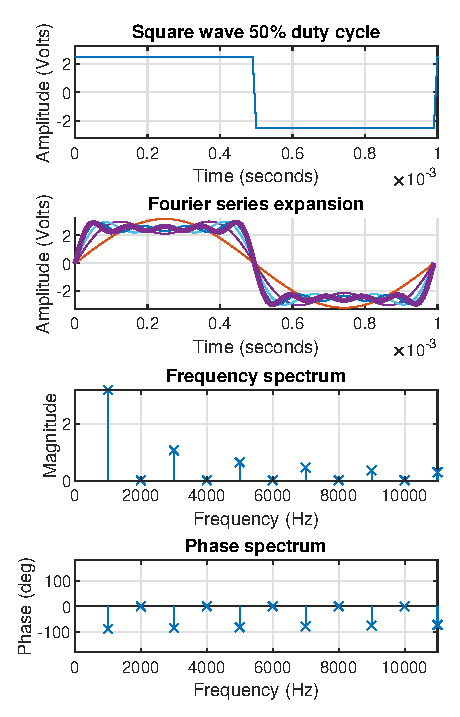
\includegraphics[width=0.3\textwidth]{../Matlab/img/sqr50}
		\caption{example plot}
		\label{fig:example-plot}
	\end{wrapfigure}
	All calculations are made using Matlab with Signal Processing Toolbox, source code can be found in Appendix \ref{sec:source-code}
	
	First step in our calculation is generating signals that we measured during exercise. Pure signals were obtained with built-in functions of Signal Processing Toolbox and Filtered signals were evaluated using NI Multisim SPICE software.
		
	Next step is finding first 10 coefficients of Fourier series for a signal which we calculated by taking inner product of signal with basis vector. In our calculations we used $\sin nt ,\thinspace \cos nt$ and $1$ as our basis vectors.
	\begin{equation}\label{eq:a0}
		a_0 = \left\langle s(t), 1 \right\rangle
	\end{equation}
	\begin{equation}\label{eq:an}
		a_n = \left\langle s(t), \cos n\omega t \right\rangle
	\end{equation}
	\begin{equation}\label{eq:bn}
		b_n = \left\langle s(t), \sin n\omega t \right\rangle
	\end{equation}

	During exercise we recorded Fourier series of a signal in Amplitude-Phase form so we need to convert $a_n$ and $b_n$ coefficients into amplitude $A_n$ and phase $\varphi_n$
	\begin{equation}\label{eq:An}
		A_n = \sqrt{a_n^2 + b_n^2}
	\end{equation}
	\begin{equation}\label{eq:phi}
		\varphi_n = \arg(a_n - j b_n)
	\end{equation}
		
	Knowing first 10 coefficients we can plot approximation of a signal using one of following formulas. Example of approximation of square wave is on the second plot in Figure \ref{fig:example-plot}.
	
	\begin{equation}\label{eq:FS}
		s(t) \approx \frac{a_0}{2} + \sum_{n=1}^{10}(a_n\cos(n\omega t)+b_n\sin(n\omega t))
	\end{equation}
	\begin{equation}\label{eq:FSap}
		s(t) \approx \frac{A_0}{2} + \sum_{n=1}^{10}(A_n\cos(n\omega t +\varphi_n))
	\end{equation}

	For third and fourth plot in Figure \ref{fig:example-plot} we are calculating Discrete Fourier transform for 10 oscillations of a signal using Fast Fourier transform algorithm from Signal Processing Toolbox and then plotting magnitude and argument of FT both in decibel scale on vertical axis.

	\section{Comparison}
	We are going to be comparing calculated and measured signals, their Fourier series expansion and/or Fourier transform. During comparison we will determine if the Harmonic analysis is useful in signal analysis and what benefits does it bring.
	
	$\ast$ Yellow signal on oscilloscope is pure signal, Blue is filtered signal
	\subsection{Pure signals}\label{sec:pure-signals}
	Starting off with first signal, Sinus, we can see that $A_n$ coefficient for 1 kHz is approximately equal to an amplitude of a signal and rest of coefficients are very small almost negligible, phase coefficient $\varphi_n$ at 1 kHz is approximately -90\degree therefore according to eq.\eqref{eq:FSap} first element of Fourier series is just $A_1 \sin \omega t$ and the rest of elements are very small, negligible.
	\begin{figure}[H]
		\centering
		\begin{subfigure}[][][t]{0.28\textwidth}
			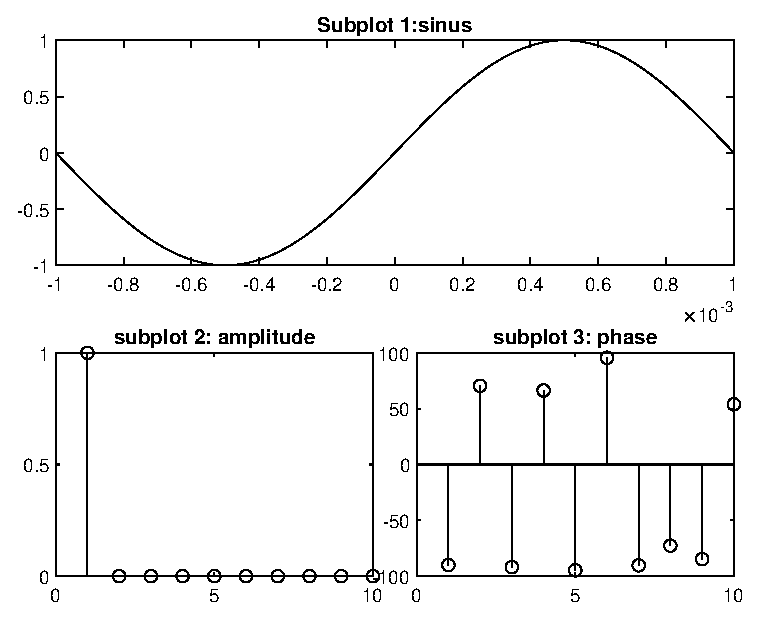
\includegraphics[width=\textwidth]{../Matlab/img/sin}
			\caption{calculated}
			\label{fig:calc-signals-a}
		\end{subfigure}
		\quad
		\begin{subfigure}[][][t]{0.28\textwidth}
			\includegraphics[width=\textwidth, trim=85 50 112 45, clip]{../img/osc/DS2_QuickPrint5.png}
			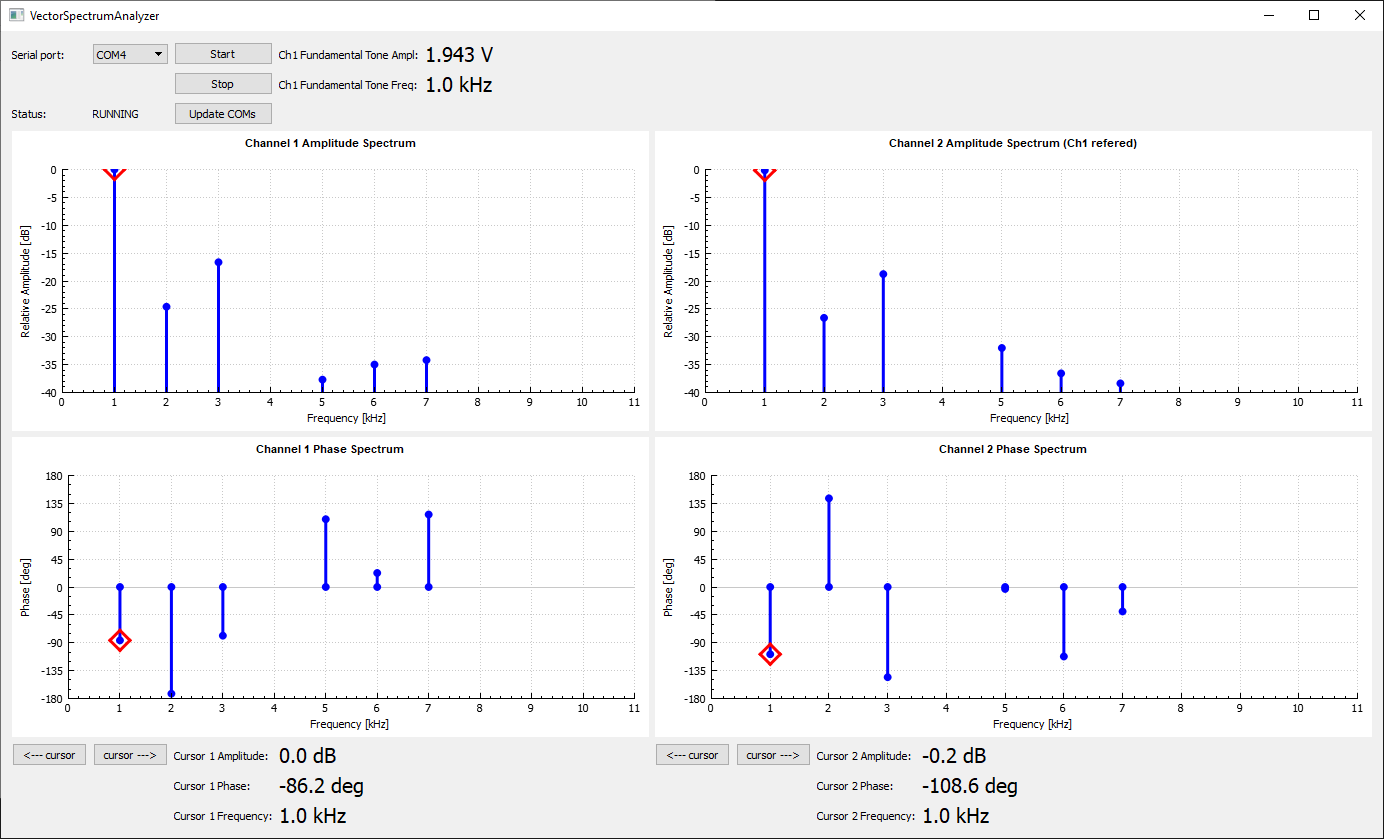
\includegraphics[width=\textwidth, trim=10 80 555 100, clip]{../img/Circuit1/sin}
			\caption{measured}
			\label{fig:meas-signal-a}
		\end{subfigure}
		\caption{Sin wave}
		\label{fig:pure-sin}
	\end{figure}
	
	Now moving to more interesting signal than simple sin, square wave, we can see many more components of Fourier series that are not negligible. Starting with first element which is exactly the same as in sin signal we can deduce that square signal have similar shape to sinus and is mostly odd function, but looking further on the rest of coefficients we can see that all non-zero coefficients are shifted by -90\degree, so the square signal is built entirely from sins and therefore is completely odd.
	
	\begin{figure}[H]
		\centering
		\begin{subfigure}[][][t]{0.28\textwidth}
			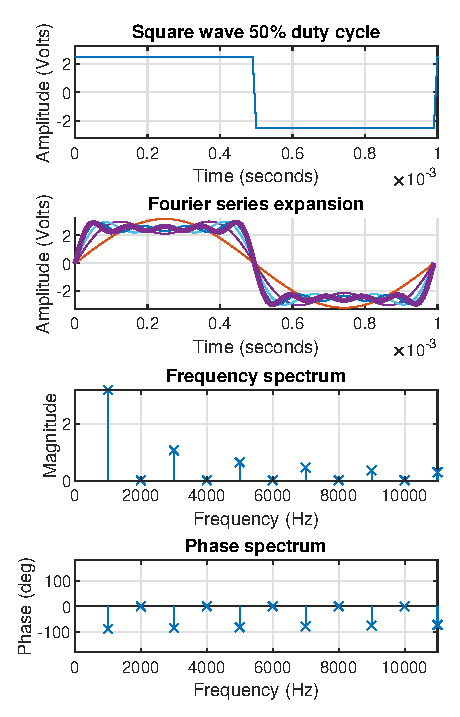
\includegraphics[width=\textwidth]{../Matlab/img/sqr50}
			\caption{calculated}
			\label{fig:calc-signals-b}
		\end{subfigure}
		\quad
		\begin{subfigure}[][][t]{0.28\textwidth}
			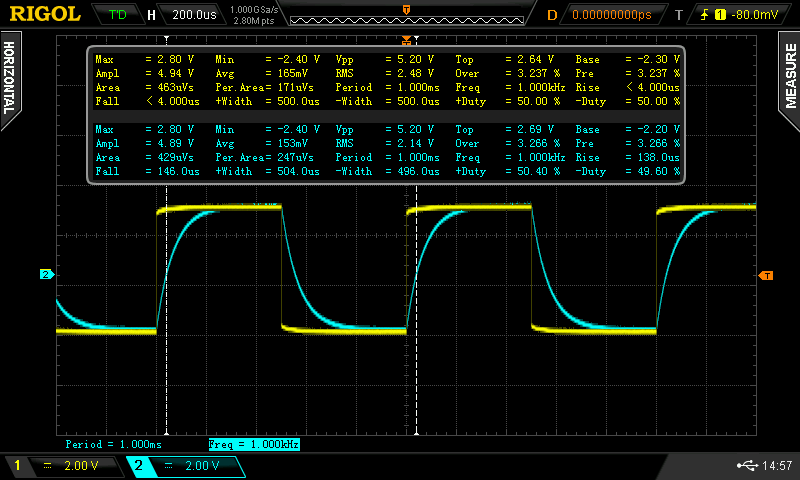
\includegraphics[width=\textwidth, trim=85 50 112 45, clip]{../img/osc/DS2_QuickPrint4.png}
			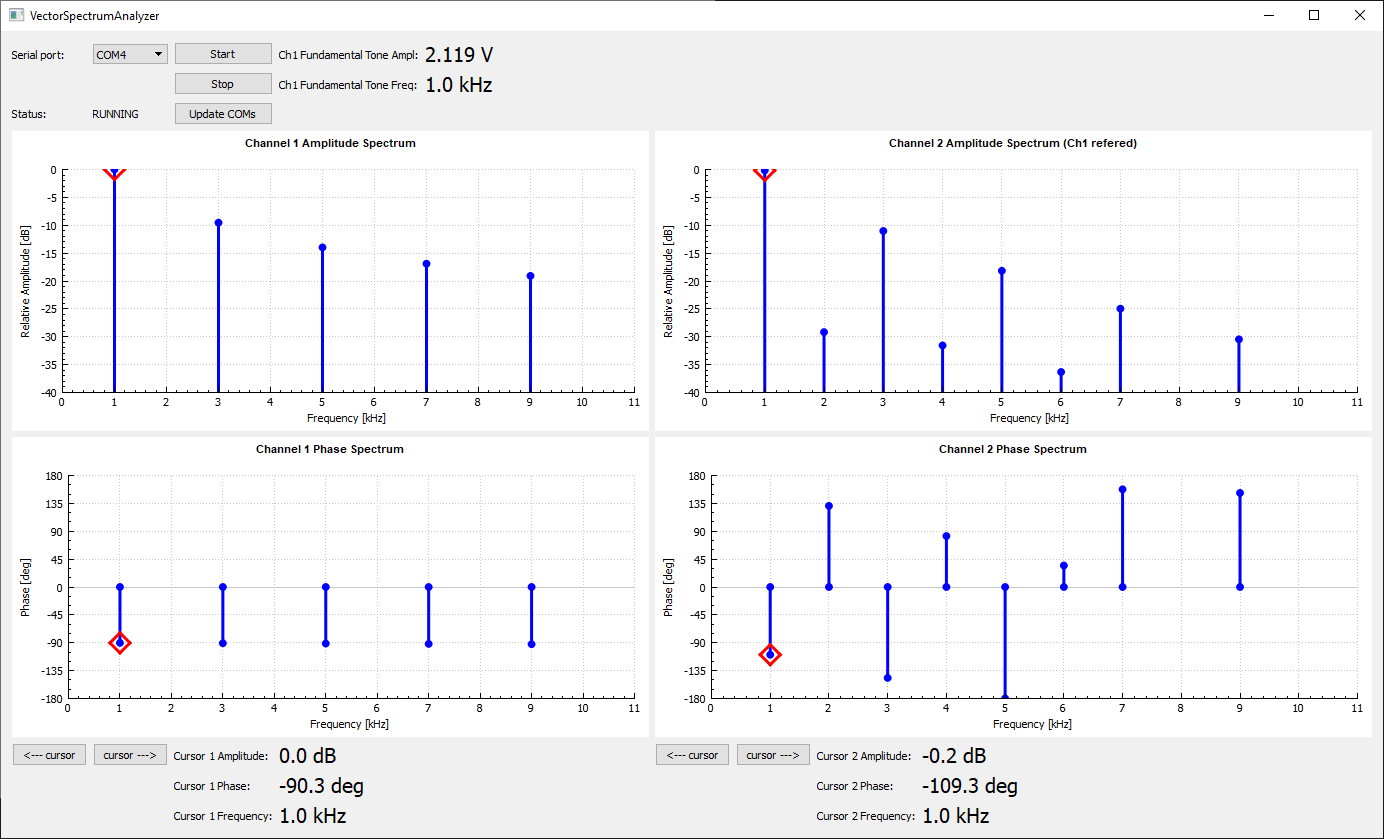
\includegraphics[width=\textwidth, trim=10 80 555 100, clip]{../img/Circuit1/dut50}
			\caption{measured}
			\label{fig:meas-signal-b}
		\end{subfigure}
		\caption{Square wave 50\% duty cycle}
		\label{fig:pure-sqr50}
	\end{figure}
	
	Third signal is also square wave but 25\% duty cycle. Looking at the most significant coefficients we can see that it is shifted by -45\degree therefore the signal is neither odd or even, also when looking at both coefficient there is repeating pattern. Phase of a harmonic is changing in order to negate previous, more significant harmonic.
	
	\begin{figure}[H]
		\centering
		\begin{subfigure}[][][t]{0.3\textwidth}
			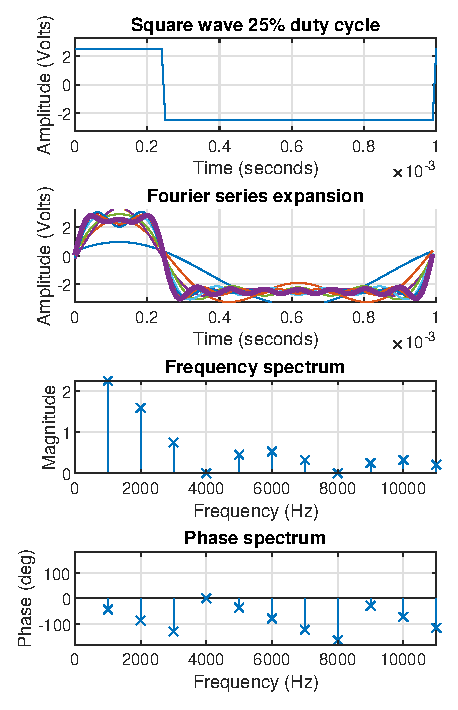
\includegraphics[width=\textwidth]{../Matlab/img/sqr25}
			\caption{calculated}
			\label{fig:calc-signals-c}
		\end{subfigure}
		\quad
		\begin{subfigure}[][][t]{0.3\textwidth}
			\includegraphics[width=\textwidth, trim=85 50 112 45, clip]{../img/osc/DS2_QuickPrint3.png}
			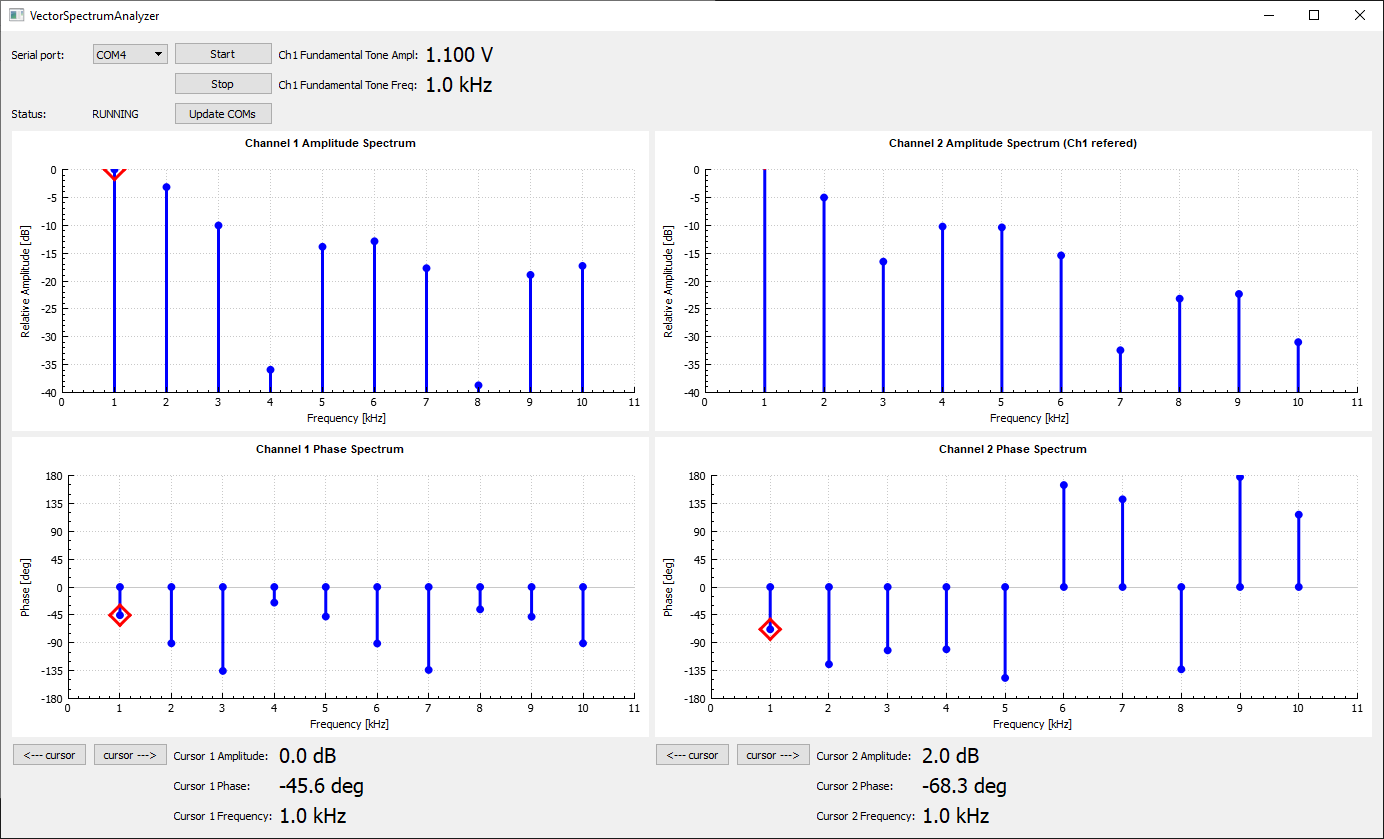
\includegraphics[width=\textwidth, trim=10 80 555 100, clip]{../img/Circuit1/dut25}
			\caption{measured}
			\label{fig:meas-signal-c}
		\end{subfigure}
		\caption{Square wave 25\% duty cycle}
		\label{fig:pure-sin}
	\end{figure}
	
	Last of the pure signals is a triangle wave, the signal is very similar to the pure sin wave, even first element is exactly the same as in sin wave, but all the differences are in harmonics with significantly smaller amplitudes that are "fine tuning" the signal.
	
	\begin{figure}[H]
		\centering
		\begin{subfigure}[][][t]{0.3\textwidth}
			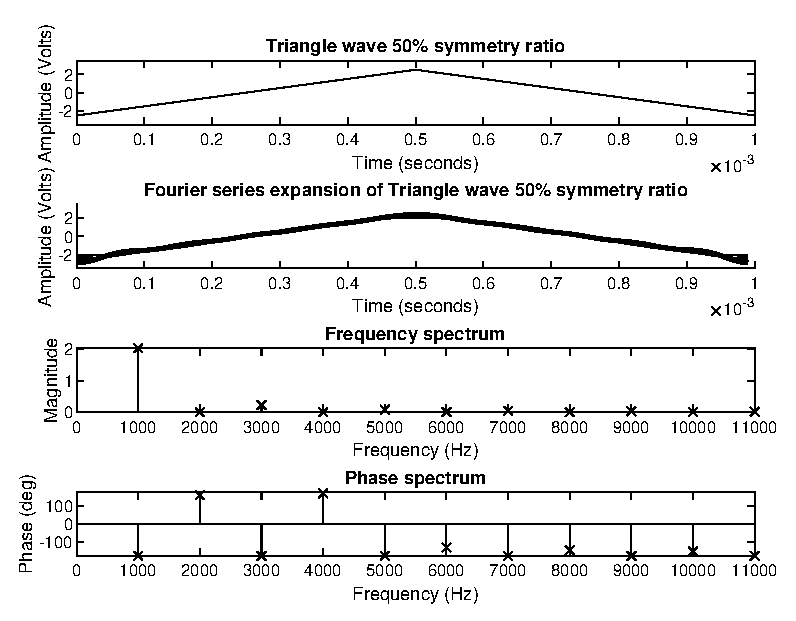
\includegraphics[width=\textwidth]{../Matlab/img/tri50}
			\caption{calculated}
			\label{fig:calc-signals-d}
		\end{subfigure}
		\quad
		\begin{subfigure}[][][t]{0.3\textwidth}
			\includegraphics[width=\textwidth, trim=85 50 112 45, clip]{../img/osc/DS2_QuickPrint2.png}
			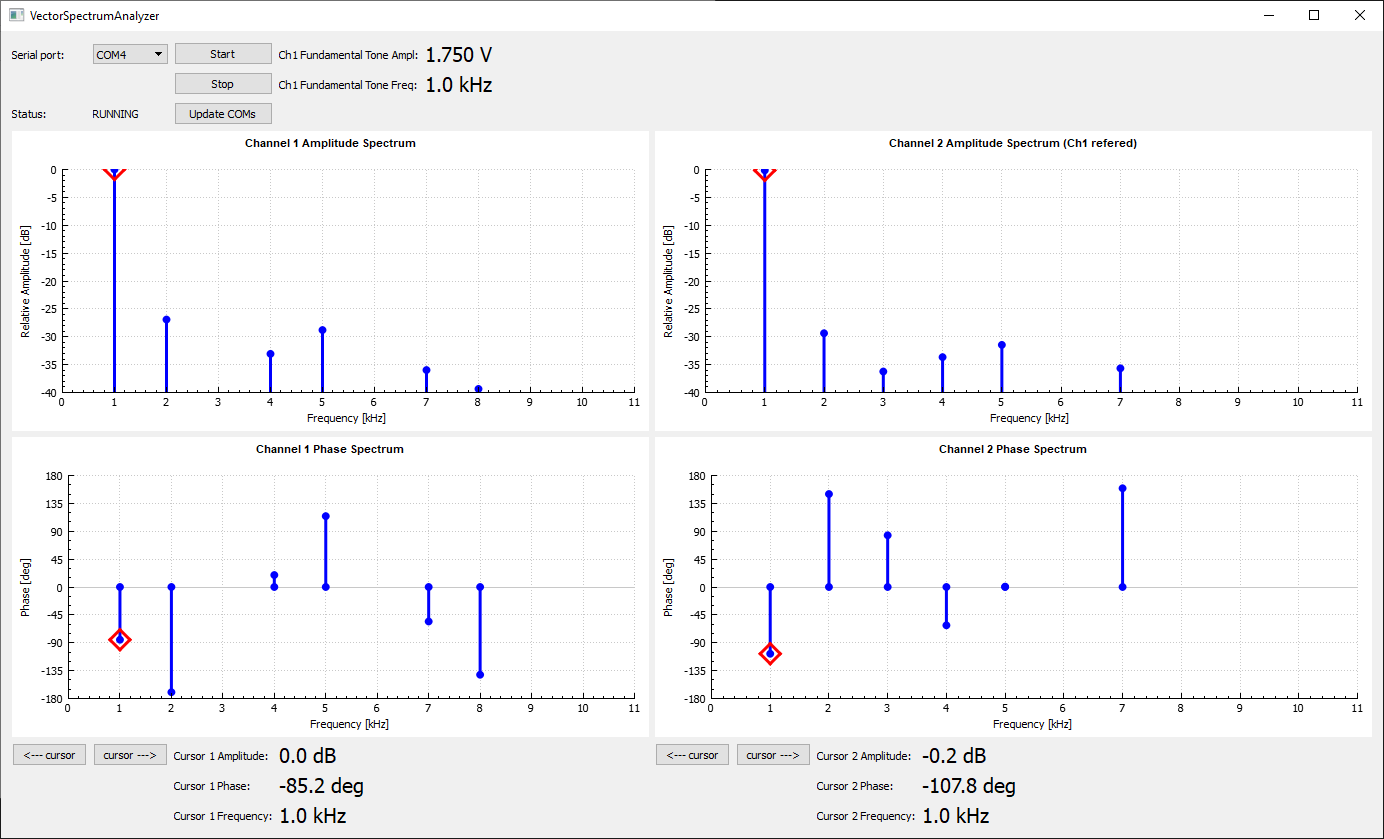
\includegraphics[width=\textwidth, trim=10 80 555 100, clip]{../img/Circuit1/trig50}
			\caption{measured}
			\label{fig:meas-signal-d}
		\end{subfigure}
		\caption{Triangle wave 50\% symmetry ratio}
		\label{fig:pure-sin}
	\end{figure}
		
	\subsection{RC filters}\label{sec:rc-filters}
	
	Simple Low-pass and High pass filters can be build with just 2 simple electric components resistor and capacitor, the reason why it is possible is that capacitor is acting differently for low frequencies and high frequencies. From formula for impedance of capacitor $\mathbf{Z}=\frac{1}{j\omega C}$ we can see that if $\omega$ is approaching 0, impedance will go to infinity therefore we can treat if like open circuit, but when $\omega$ is approaching infinity, impedance will go to 0 so capacitor will act like a wire.
	
		\begin{figure}[H]
		\centering
		\begin{subfigure}{0.45\textwidth}
			\centering
			\begin{circuitikz}[scale = 0.7, transform shape]
				\draw (0,0) node[bnc](B1) {}
				to[R, l=$R_{11}$, a=1.5k$\Omega$] (3,0)
				to[C, l=$C_{11}$, a=47nF] (3,-2)
				node[ground] {}
				;
				\draw (3,0) 
				to[short] (4.5,0)
				node[bnc, xscale=-1](B2){\scalebox{-1}[1]{}}
				;
				\draw node[ground] at (B1.shield) {};
				\draw node[ground] at (B2.shield) {};
			\end{circuitikz}
			\caption{Low-pass filter}
			\label{fig:filter-a}
		\end{subfigure}
		\begin{subfigure}{0.45\textwidth}
			\centering
			\begin{circuitikz}[scale = 0.7, transform shape]
				\draw (0,0) node[bnc](B1) {}
				to[C, l=$C_{21}$, a=10nF] (3,0)
				to[R, l=$R_{21}$, a=\tiny1.5k$\Omega$] (3,-2)
				node[ground] {}
				;
				\draw (3,0) 
				to[short] (4.5,0)
				node[bnc, xscale=-1](B2){\scalebox{-1}[1]{}}
				;
				\draw node[ground] at (B1.shield) {};
				\draw node[ground] at (B2.shield) {};
			\end{circuitikz}
			\caption{High-pass filter}
			\label{fig:filter-b}
		\end{subfigure}
		\caption{RC filters}
		\label{fig: Filters}
	\end{figure}
	
	\subsubsection{Low-pass filter}

	First signal that we filtered using low-pass filter and measured was square wave 50\% duty cycle. The most notable thing in the comparison of unfiltered and filtered signals is that the amplitudes of harmonics with smaller frequency barely change when those with higher frequencies are changed by several decibels.

	\begin{figure}[H]
		\centering
		\begin{subfigure}[][][t]{0.26\textwidth}
			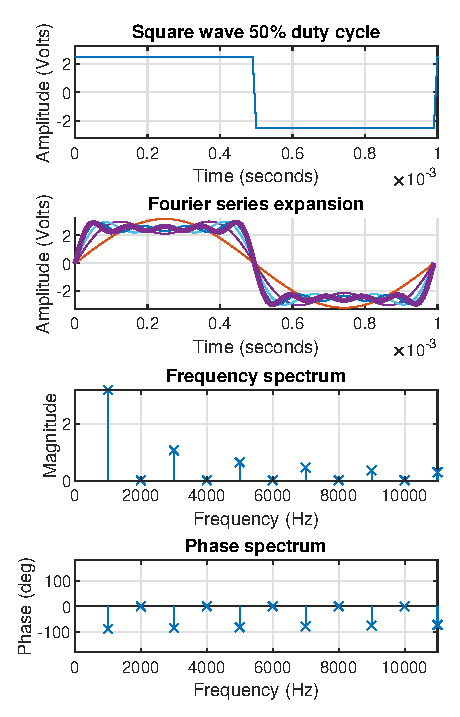
\includegraphics[width=\textwidth]{../Matlab/img/sqr50}
			\caption{Pure signal}
		\end{subfigure}
		\hfill
		\begin{subfigure}[][][t]{0.26\textwidth}
			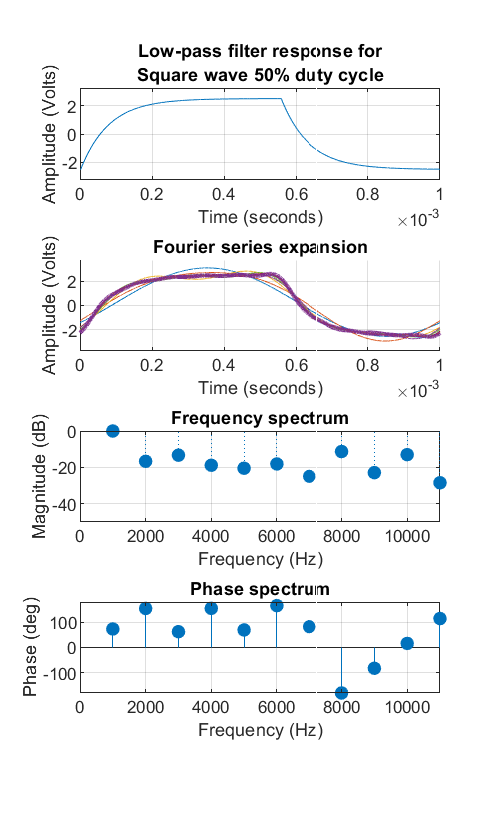
\includegraphics[width=\textwidth]{../Matlab/img/RCLPsqr50}
			\caption{Filtered signal}
		\end{subfigure}
		\hfill
		\begin{subfigure}[][][t]{0.45\textwidth}
			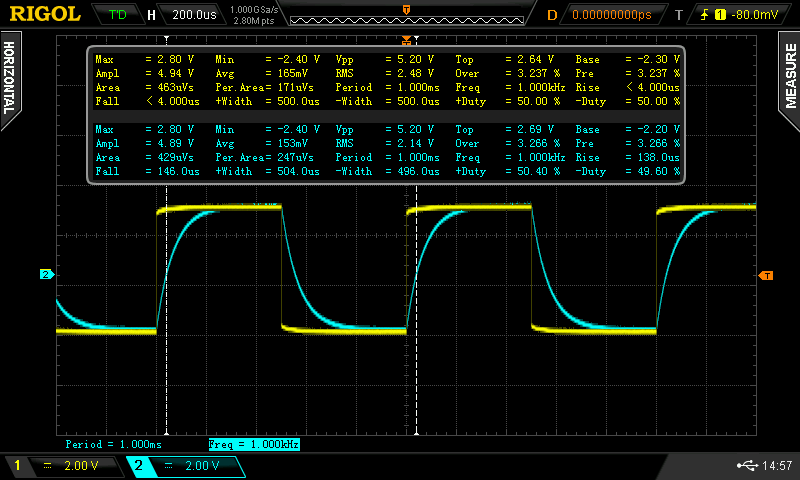
\includegraphics[width=\textwidth, trim=85 50 112 45, clip]{../img/osc/DS2_QuickPrint4.png}
			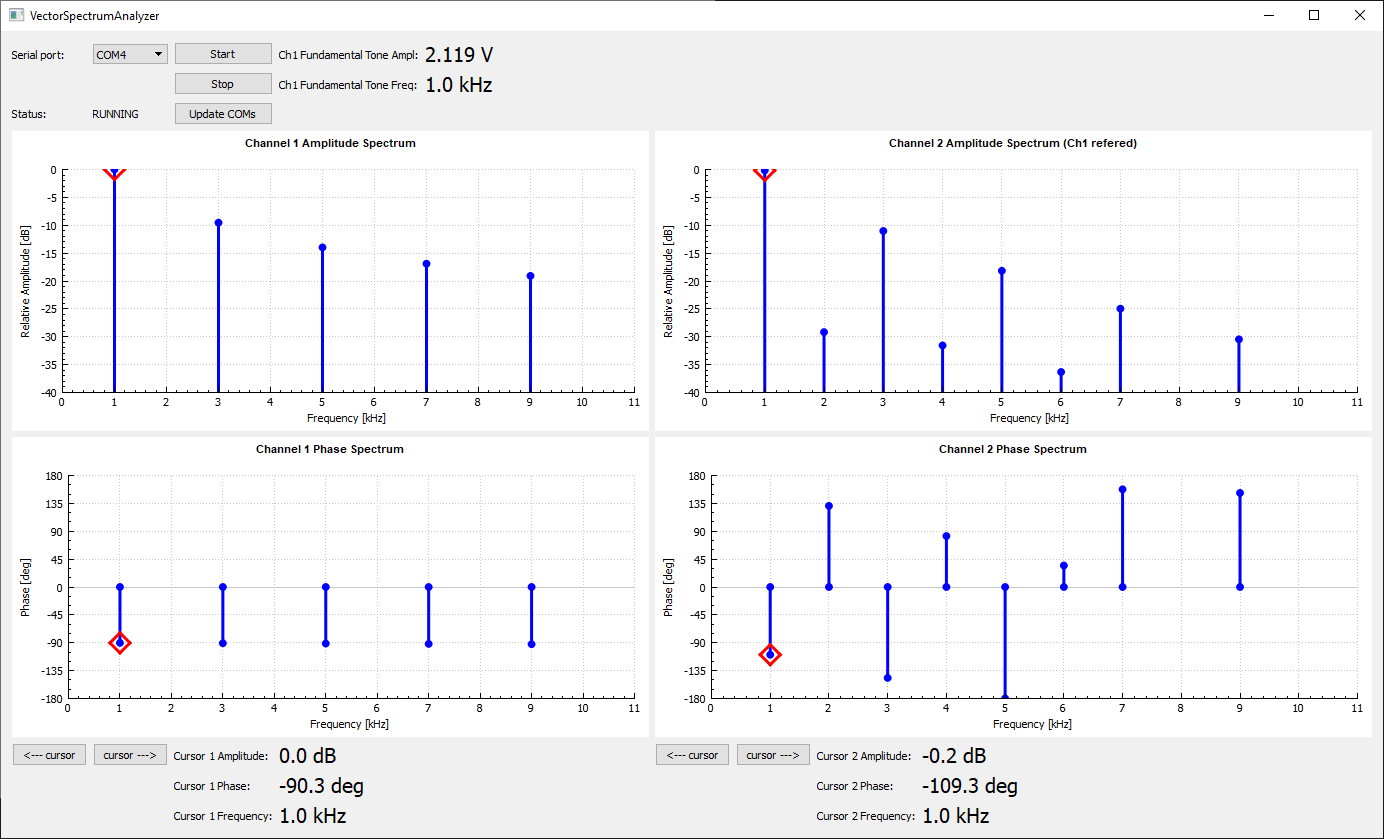
\includegraphics[width=\textwidth, trim=10 80 10 100, clip]{../img/Circuit1/dut50}
			\caption{Measured signal}
		\end{subfigure}
		\caption{Low-pass filter response for Square wave 50\% duty cycle}
	\end{figure}
	
	\newpage
	
	For filtered triangle wave 40\% duty cycle similar to square wave amplitudes of harmonics with higher frequency are decreased by few decibels, and without those higher frequency harmonics which are responsible for "thin tuning" of signal loses sharp shape and retains rough shape of the signal.
	
	\begin{figure}[H]
		\centering
		\begin{subfigure}[][][t]{0.26\textwidth}
			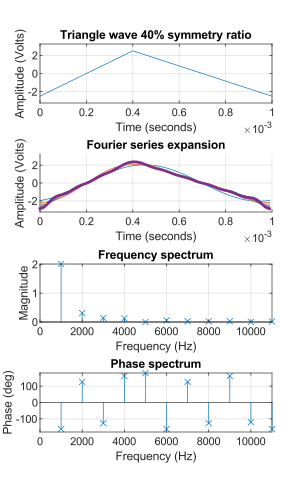
\includegraphics[width=\textwidth]{../Matlab/img/tri40}
			\caption{Pure signal}
		\end{subfigure}
		\hfill
		\begin{subfigure}[][][t]{0.26\textwidth}
			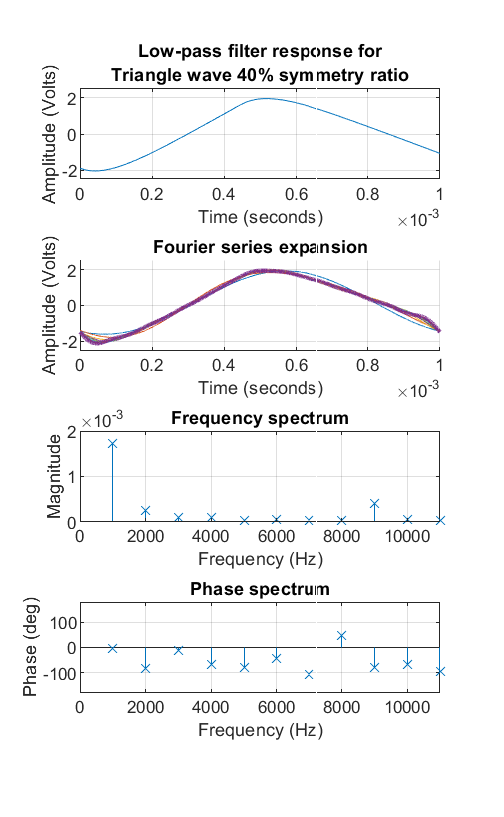
\includegraphics[width=\textwidth]{../Matlab/img/RCLPtri40}
			\caption{Filtered pure signal}
		\end{subfigure}
		\hfill
		\begin{subfigure}[][][t]{0.45\textwidth}
			\includegraphics[width=\textwidth, trim=85 50 112 45, clip]{../img/osc/DS2_QuickPrint1.png}
			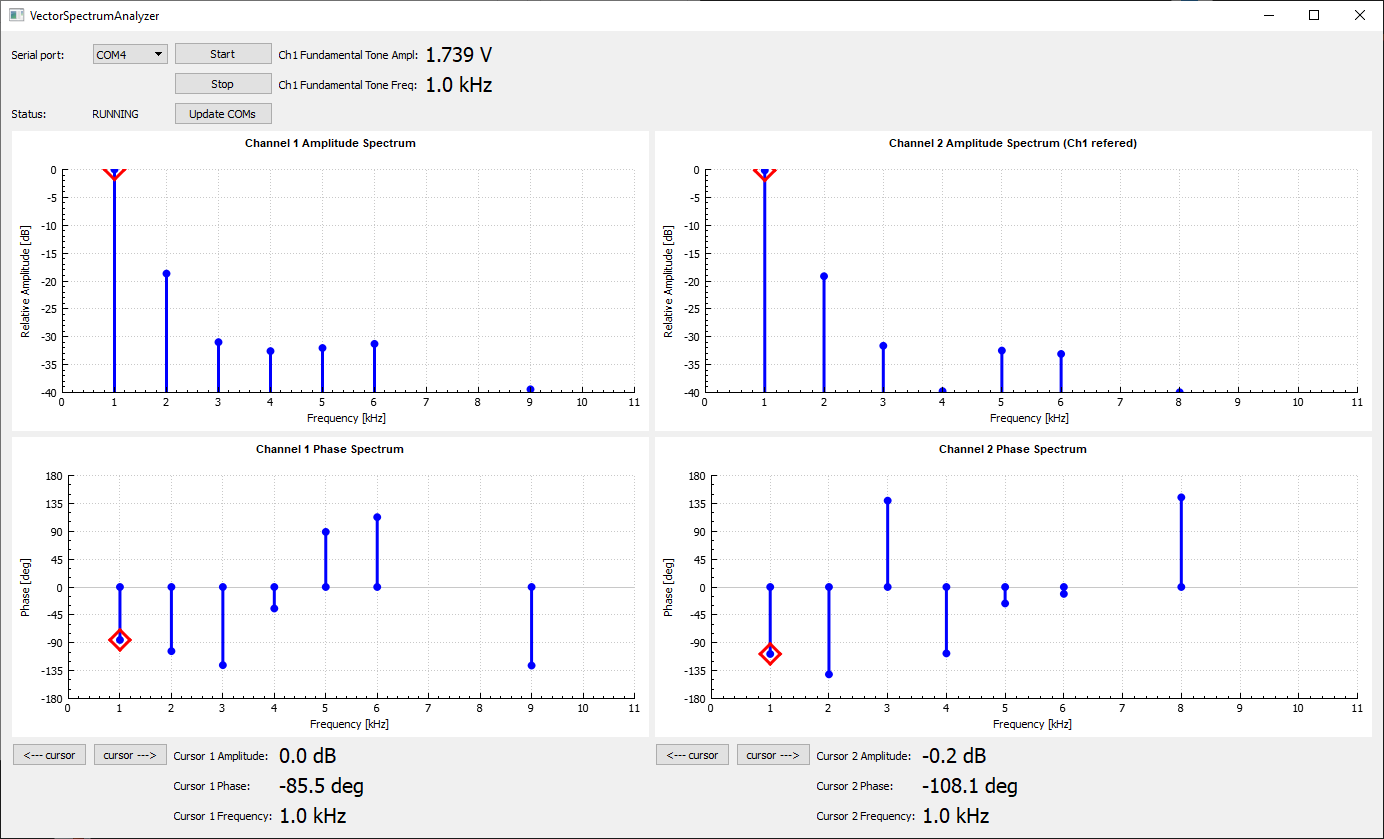
\includegraphics[width=\textwidth, trim=10 80 10 100, clip]{../img/Circuit1/trig40}
			\caption{Measured signal}
		\end{subfigure}
		\caption{Low-pass filter response for Triangle wave 40\% symmetry ratio}
	\end{figure}
	
	\subsubsection{High-pass filter}
	
	Moving to High-pass filter we measured the same signals as in Low-pass filter. Starting with the square wave. Looking at amplitudes we can see that only small frequency harmonics are greatly impacted by order of -20dB which is around 0.1 of original amplitude, decrease of the amplitudes of harmonics eases off with increasing frequency.
	
	\begin{figure}[H]
		\centering
		\begin{subfigure}[][][t]{0.26\textwidth}
			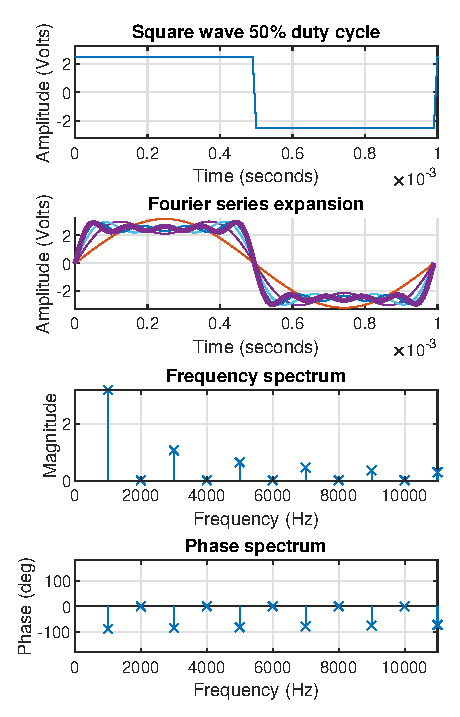
\includegraphics[width=\textwidth]{../Matlab/img/sqr50}
			\caption{Pure signal}
		\end{subfigure}
		\hfill
		\begin{subfigure}[][][t]{0.26\textwidth}
			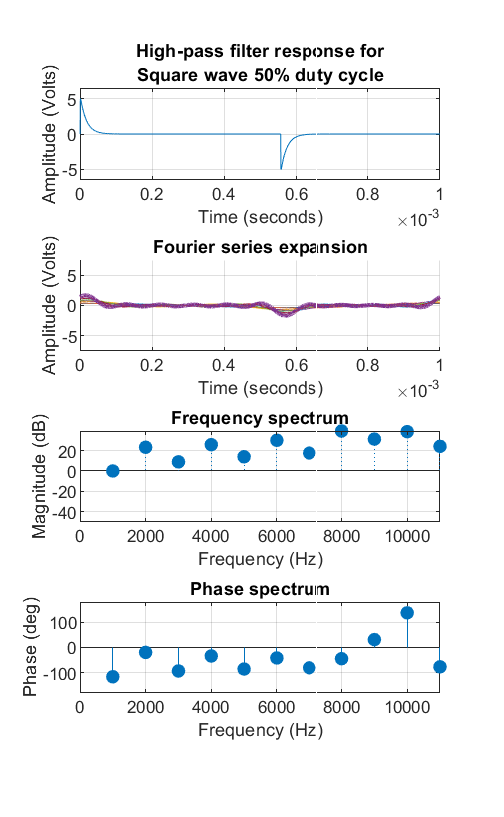
\includegraphics[width=\textwidth]{../Matlab/img/RCHPsqr50}
			\caption{Filtered pure signal}
		\end{subfigure}
		\hfill
		\begin{subfigure}[][][t]{0.45\textwidth}
			\includegraphics[width=\textwidth, trim=85 50 112 45, clip]{../img/osc/DS2_QuickPrint7.png}
			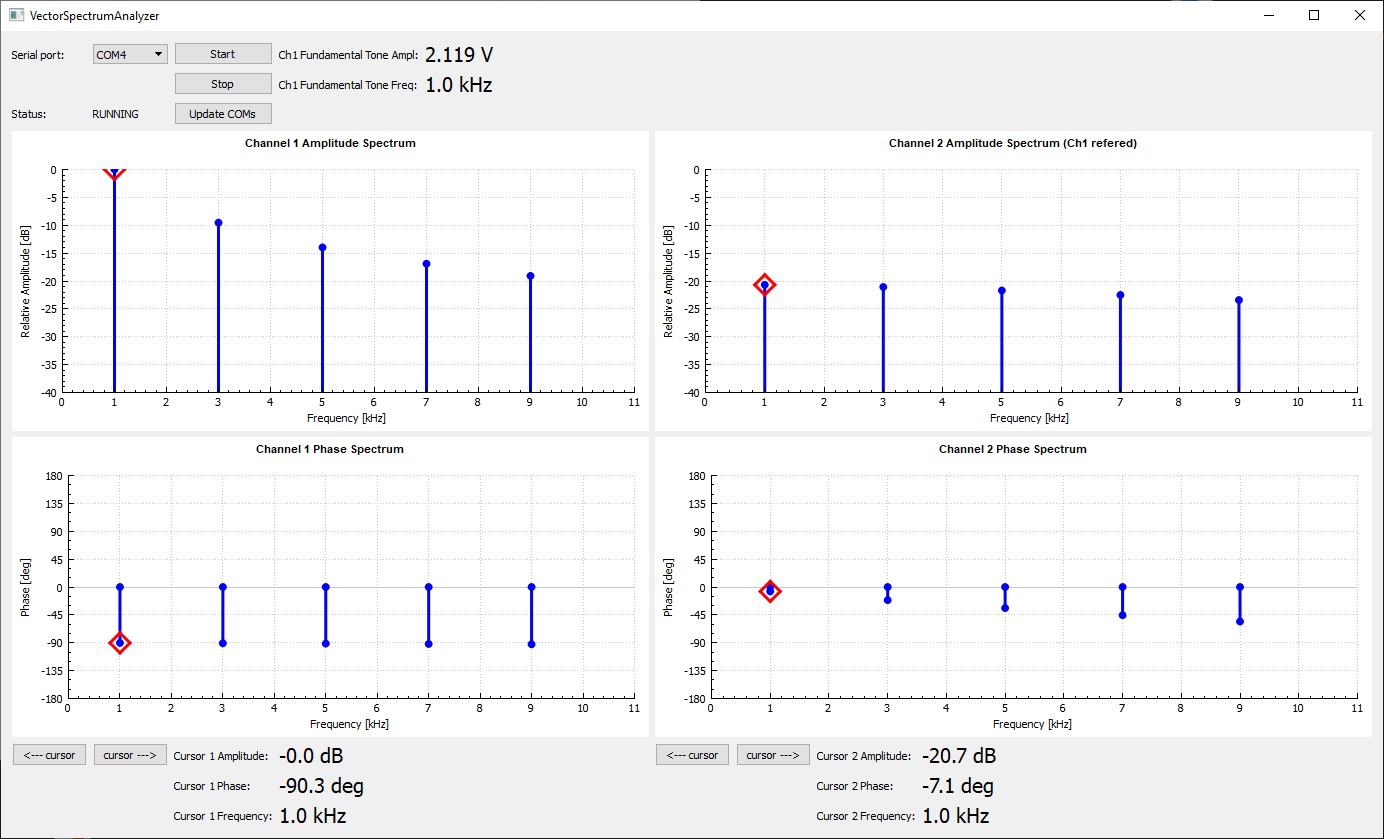
\includegraphics[width=\textwidth, trim=10 80 10 100, clip]{../img/Circuit2/dut50}
			\caption{Measured signal}
		\end{subfigure}
		\caption{Low-pass filter response for Square wave 50\% duty cycle}
	\end{figure}
	
	Moving to last of the signals which is Triangle wave with 40\% symmetry ratio. Similar to previous case the biggest difference is in first harmonic with lowest frequency, amplitude is reduced by -20dB another thing is change in phase between filtered and unfiltered first harmonic. Phase of first harmonic change to better match extremes of filtered signal.
	
	\begin{figure}[H]
		\centering
		\begin{subfigure}[][][t]{0.26\textwidth}
			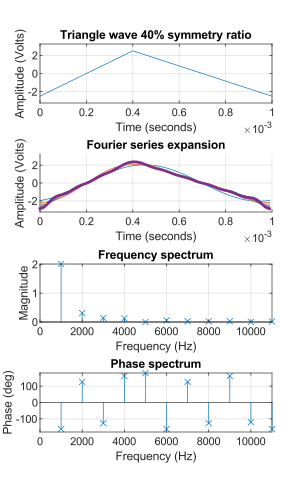
\includegraphics[width=\textwidth]{../Matlab/img/tri40}
			\caption{Pure signal}
		\end{subfigure}
		\hfill
		\begin{subfigure}[][][t]{0.26\textwidth}
			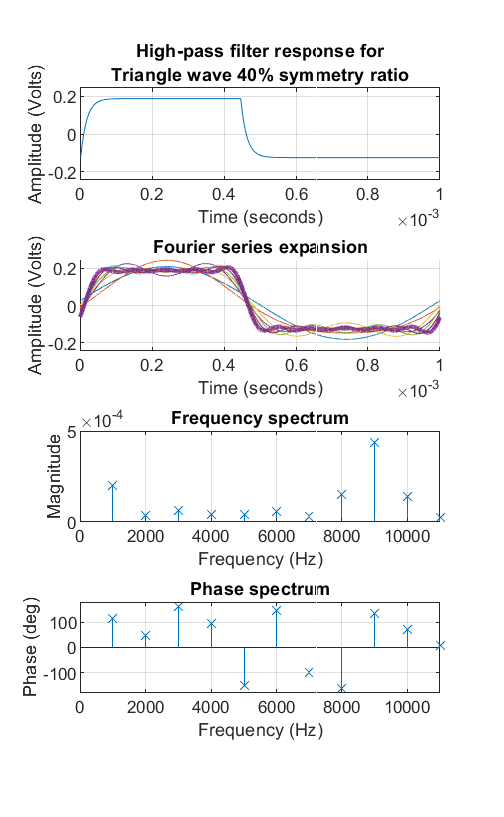
\includegraphics[width=\textwidth]{../Matlab/img/RCHPtri40}
			\caption{Filtered pure signal}
		\end{subfigure}
		\hfill
		\begin{subfigure}[][][t]{0.45\textwidth}
			\includegraphics[width=\textwidth, trim=85 50 112 45, clip]{../img/osc/DS2_QuickPrint10.png}
			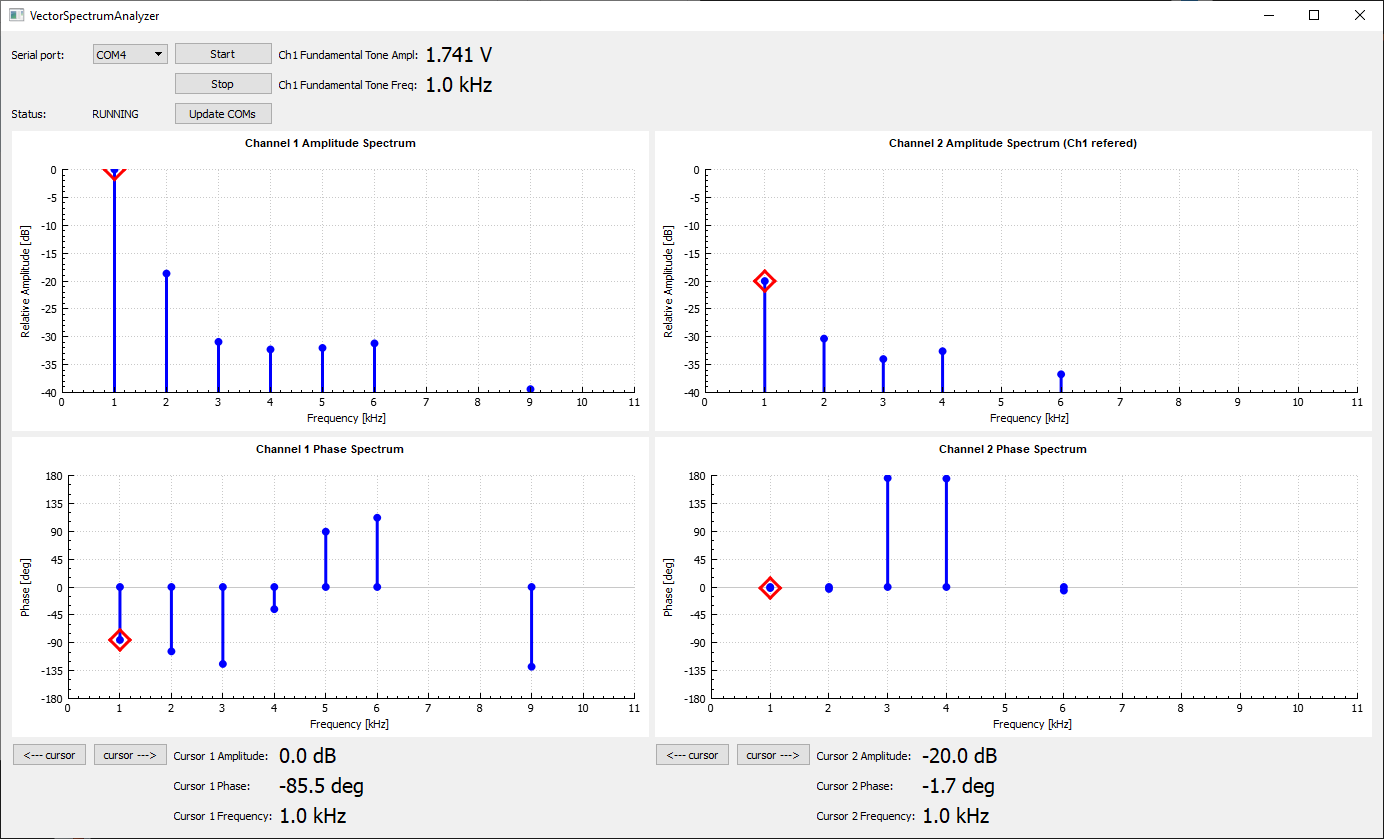
\includegraphics[width=\textwidth, trim=10 80 10 100, clip]{../img/Circuit2/trig40}
			\caption{Measured signal}
		\end{subfigure}
		\caption{Low-pass filter response for Square wave 50\% duty cycle}
	\end{figure}
	
	\section{Conclusion}
	
	Fourier series is powerful tool in signal analysis. It allows us to split signals into much simpler components and point out characteristics of more complex periodic signals, as we did in section. \ref{sec:pure-signals}. Splitting signals into simple harmonics also allows us to evaluate effectiveness of for example filters, by comparing Fourier series expansion of filtered and unfiltered signals. Another application of Fourier series which we didn't utilize is splitting the signal into sins and cosines, performing some calculation on simple function and then recombining new sines and cosines to get processed signal. For example instead of simulating RC filters' responses we could have calculated transfer functions for cosine and decompose each signal, then apply transfer function and recompose back to get output signal.
	
	\newpage
	\appendix
	\section{Source Code}\label{sec:source-code}
	\href{https://github.com/kamilix2003/CT_labs}{GITHUB repository}
	\subsection*{lab2.m}
	\inputminted{matlab}{../Matlab/lab2.m}
	\subsection*{Final Plots.m}
	\inputminted{matlab}{../Matlab/Final_Plots.m}
%	\subsection*{Fourier.m}
%	\inputminted{matlab}{../Matlab/Fourier.m}
%	\subsection*{fourier coefficient.m}
%	\inputminted{matlab}{../Matlab/fourier_coefficient.m}
	\subsection*{Import csv.m}
	\inputminted{matlab}{../Matlab/RC_circuit.m}
\end{document}
